\documentclass{BHCexam}

\begin{document}
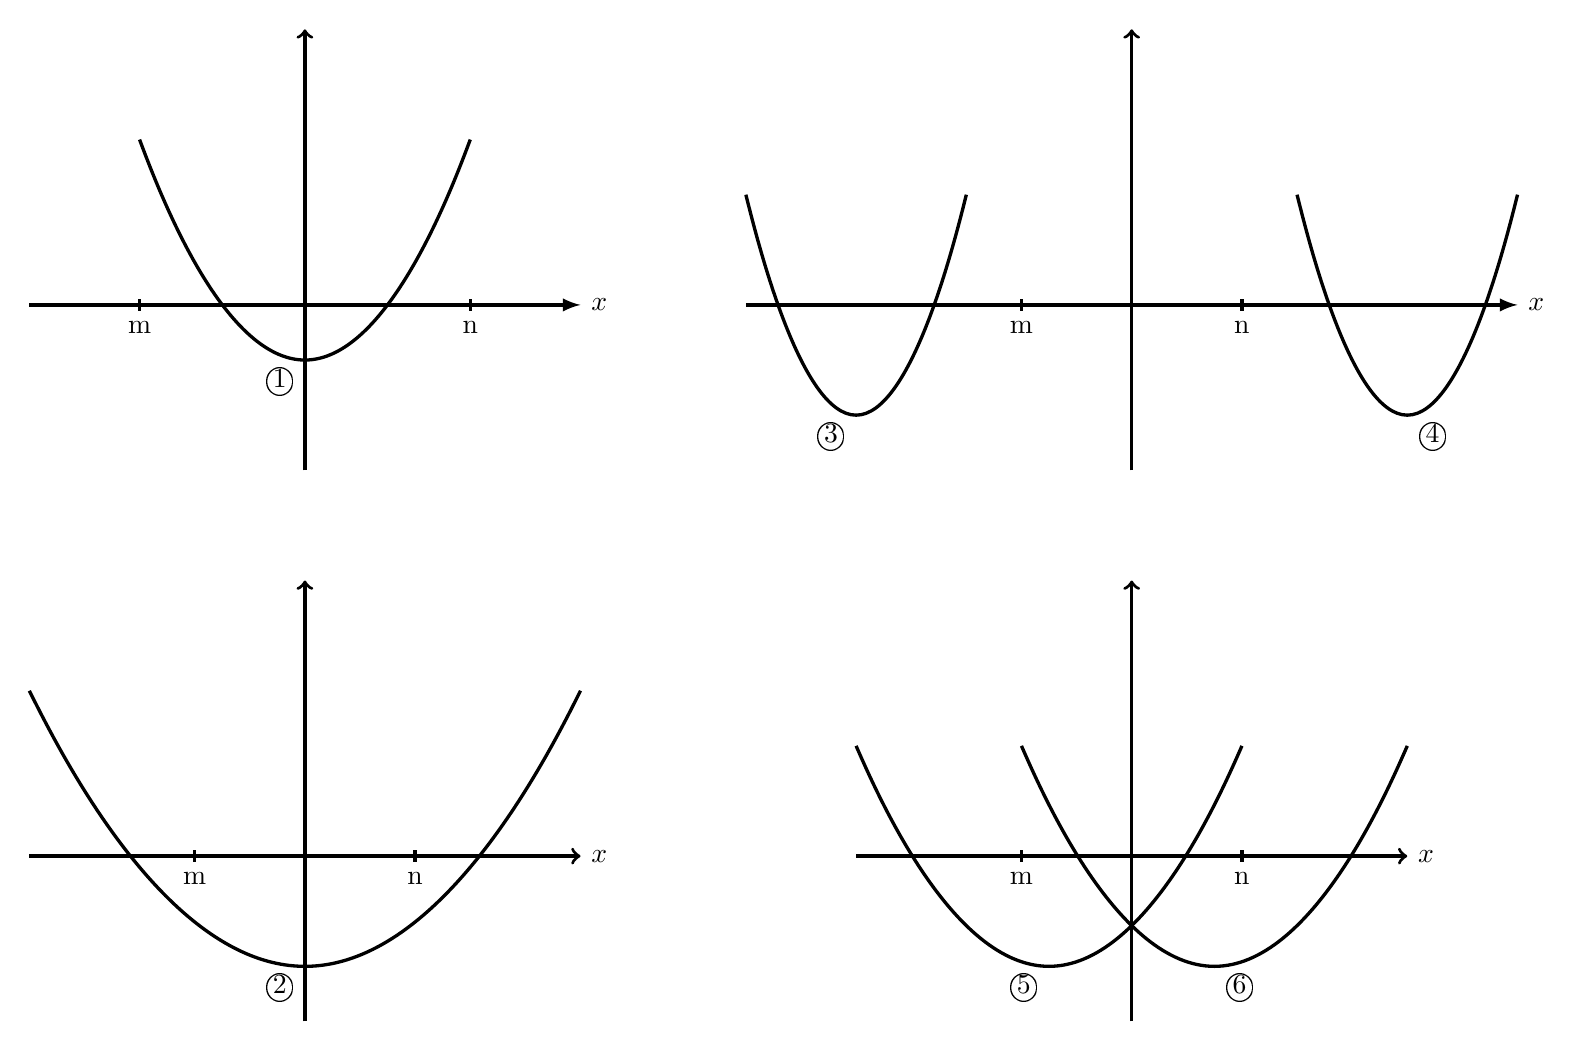
\begin{tikzpicture}[scale=0.7]
 
 
\draw[->,>=latex,very thick] (-5,0) --(5,0) node[right]{$x$};
\draw[->,very thick] (0,-3) --(0,5);
\draw[very thick ] (-3,3) parabola bend (0,-1)  (3,3);
\draw node [below left] at (0,-1) {\textcircled{$1$}};
 
\foreach \x/\xtext in {-3/$m$,3/$n$}
\draw[shift={(\x,0)},very thick] (0pt,3pt) -- (0pt,-3pt) node[below] {$\xtext$};
 
\begin{scope}[yshift=-10cm]
\draw[->,very thick] (-5,0) --(5,0) node[right]{$x$};
\draw[->,very thick] (0,-3) --(0,5);
\draw[very thick ] (-5,3) parabola bend (0,-2) (5,3);
\draw node [below left] at (0,-2) {\textcircled{$2$}};
 
\foreach \x/\xtext in {-2/$m$,2/$n$}
\draw[shift={(\x,0)},very thick] (0pt,3pt) -- (0pt,-3pt) node[below] {$\xtext$};
\end{scope}
 
\begin{scope}[xshift=15cm]
\draw[->,>=latex,very thick] (-7,0) --(7,0) node[right]{$x$};
\draw[->,very thick] (0,-3) --(0,5);
\draw[very thick ] (-7,2) parabola[bend pos=0.5] bend +(0,-4) (-3,2);
\draw[very thick,xshift=10cm ] (-7,2) parabola[bend pos=0.5] bend +(0,-4) (-3,2);
\draw node [below left] at (-5,-2) {\textcircled{$3$}};
\draw node [rectangle,below right] at (5,-2) {\textcircled{$4$}};
 
 
\foreach \x/\xtext in {-2/$m$,2/$n$}
\draw[shift={(\x,0)},very thick] (0pt,3pt) -- (0pt,-3pt) node[below] {$\xtext$};
\end{scope}
 
\begin{scope}[xshift=15cm,yshift=-10cm]
\draw[->,very thick] (-5,0) --(5,0) node[right]{$x$};
\draw[->,very thick] (0,-3) --(0,5);
\draw[very thick ] (-5,2) parabola[bend pos=0.5] bend +(0,-4) (2,2);
\draw[very thick,xshift=3cm ]  (-5,2) parabola[bend pos=0.5] bend +(0,-4) (2,2);
\draw node [below left] at (-1.5,-2) {\textcircled{$5$}};
\draw node [below right] at (1.5,-2) {\textcircled{$6$}};
 
 
 
\foreach \x/\xtext in {-2/$m$,2/$n$}
\draw[shift={(\x,0)},very thick] (0pt,3pt) -- (0pt,-3pt) node[below] {$\xtext$};
\end{scope}
\end{tikzpicture}
\end{document}